\begin{figure*}[t]
\centering
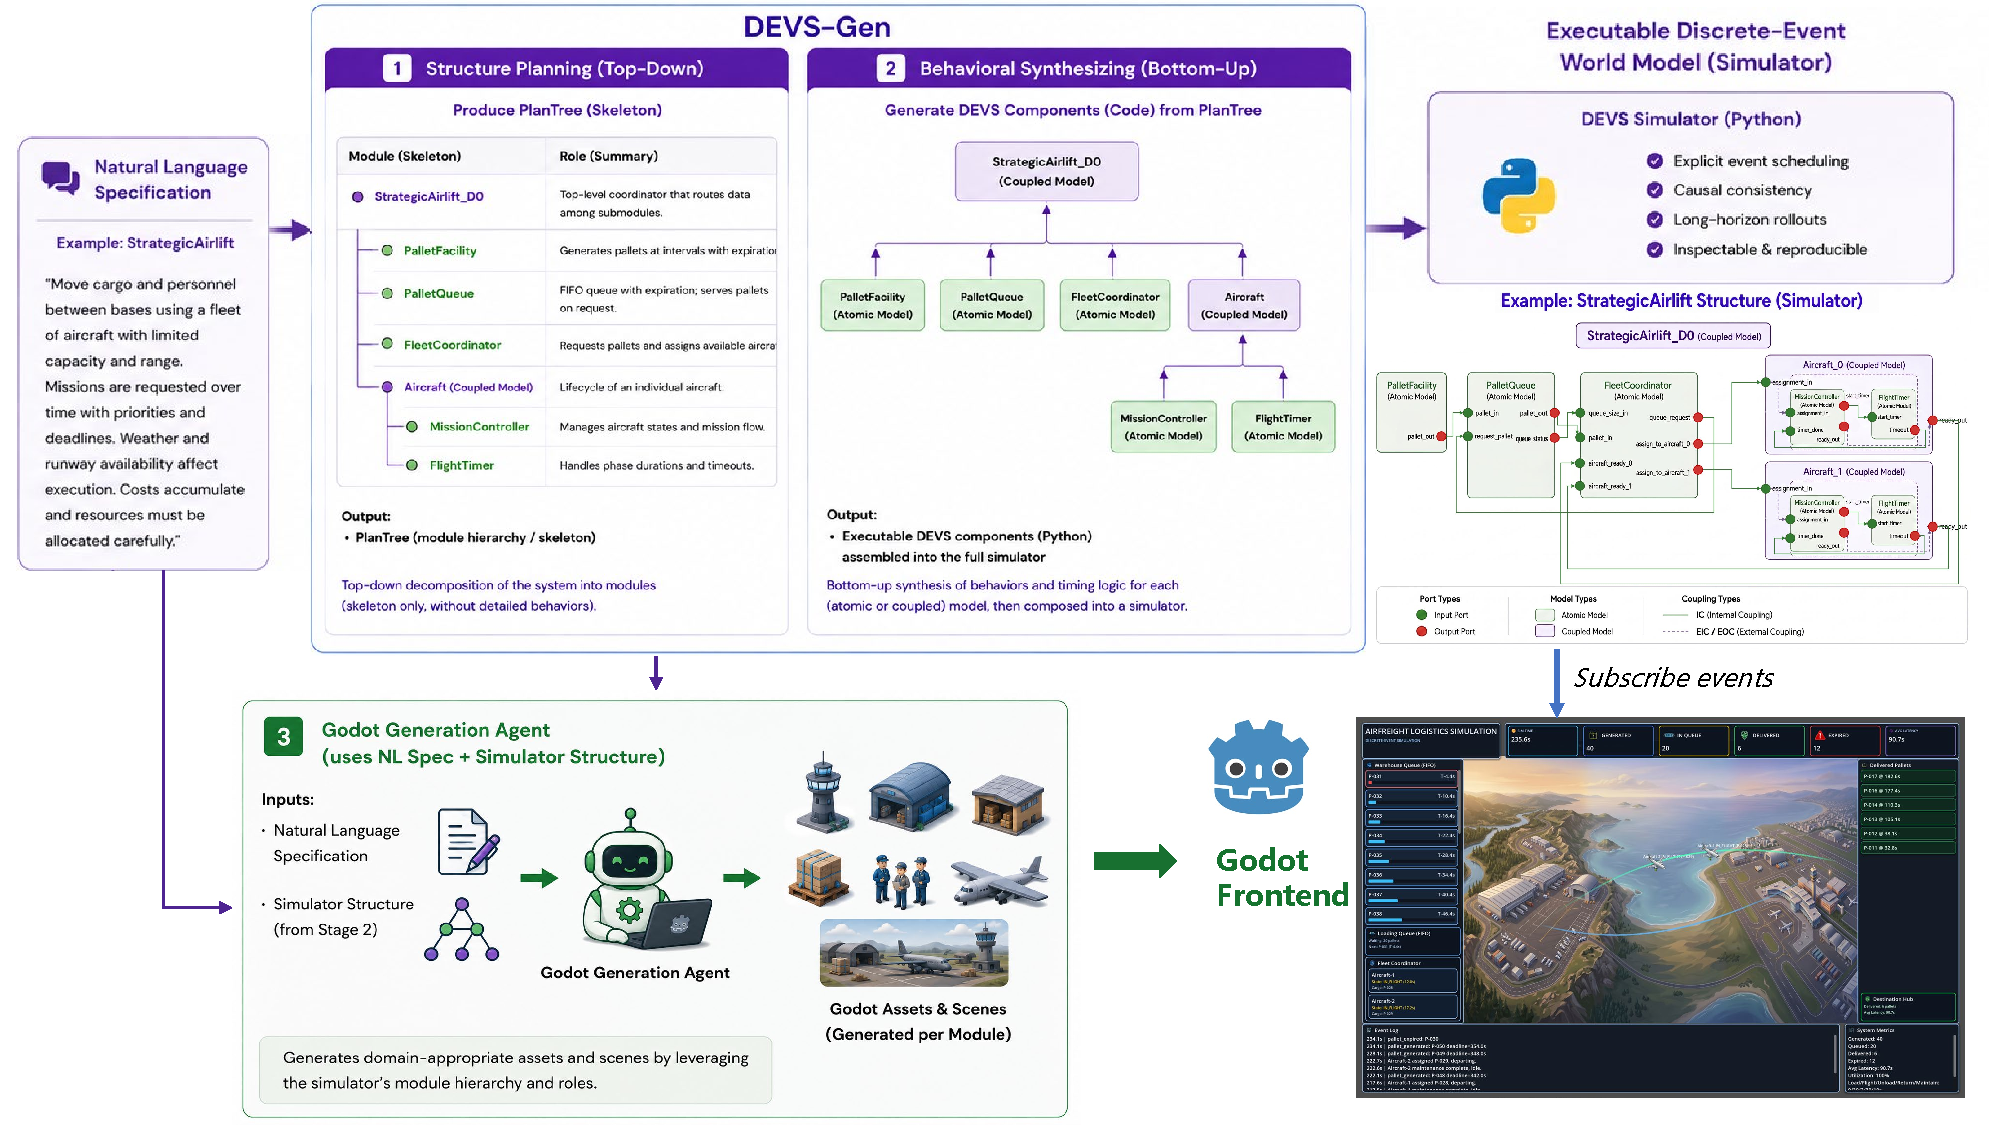
\includegraphics[width=\textwidth]{imgs/pipeline.pdf}
% \caption{Generation pipeline of the discrete-event world model, including \methodname{} and Godot.}
\caption{Illustration of \methodname. A natural-language specification is transformed into a discrete-event world model via a two-stage pipeline; its generated artifacts, including the model hierarchy and event stream, can be used to build visualization frontends for animation and interactive inspection.}
\label{fig:model_generation}
\end{figure*}

\section{DEVS-Based Model Generation Pipeline}\label{sec:method_generation}

Building on the DEVS formalization in Section~\ref{sec:preliminary}, we introduce \methodname, a pipeline for synthesizing an executable discrete-event simulator $\cM$ from a specification \spec{}. The key idea is to use DEVS as a structural scaffold: rather than generating the simulator monolithically, \methodname decomposes synthesis into a sequence of well-scoped sub-tasks. 
% The prompts used throughout the pipeline are provided in App.~\ref{app:prompts}. 
% examples of the generated simulator are provided in App.~\ref{app:code_prompt} and App.~\ref{app:artifacts_code}.
As formalized in Algorithm~\ref{alg:devs_main}, \methodname constructs $\cM$ in two stages. First, \emph{structural planning} derives an architectural \plantree{} from \spec, which assigns each component a local \modelplan{}. Second, \emph{behavioral synthesis} implements each component according to its assigned \modelplan{} and assembles the resulting modules into the final simulator. The upper half of Figure~\ref{fig:model_generation} illustrates this procedure using the warehouse robot fleet restocking example.

The central intermediate representation connecting these two stages is the \plantree{}, a hierarchical blueprint that specifies the simulator topology, assigns model types, either coupled or atomic, and defines port-based interaction contracts between models. Each node corresponds to an environment component, such as a robot, charger, or order queue, and is associated with a component-specific \modelplan{}. This acts as a local contract: it specifies the node's model type, input and output port schemas, state variables, event and timing logic, and, for coupled models, the interaction graph over its child components.

All functional operations in the pipeline (e.g., structural drafting, interface routing, and code synthesis) are implemented through specific LLM prompt templates. The prompt templates used for these operations are provided in Appendix~\ref{app:prompts}.

\begin{algorithm}[h]
\caption{\methodname{} Pseudocode}
\label{alg:devs_main}
\begin{algorithmic}[1]
\State \textbf{Input:} specification \spec
\State \textbf{Output:} simulator $\cM$ (DEVS coupled model)

\State \texttt{PlanTree} $\leftarrow$ \textsc{Plan}(\spec) \textit{// See Alg.~\ref{alg:devs_planning}}

\State $\cM \leftarrow$ \textsc{Construct}(\plantree) \textit{// See Alg.~\ref{alg:devs_construct}}

\end{algorithmic}
\end{algorithm}

\subsection{Stage 1: Structural Planning}
Stage 1 transforms \spec{} into \plantree{}. 
To control complexity, this stage is decomposed into the following two steps.
% : system skeleton drafting and local architectural refinement.

\noindent\textbf{System Skeleton Drafting.} 
Given only \spec{} as input (see App.~\ref{app:artifacts_input}), the pipeline first extracts the system's high-level structure as a \texttt{Skeleton} (see App.~\ref{app:planning_skeleton_artifact}). This artifact captures the global topology by identifying the required modules, organizing coupled models into a parent-child hierarchy, and assigning each entity a concise functional description. The resulting skeleton provides a shared architectural frame that anchors all subsequent steps.

\noindent\textbf{Architecture Refinement and Sub-tasks.}
% Guided by the \texttt{Skeleton}, the planner traverses the topology and expands each bare node into a detailed \modelplan{}. For each coupled model, the corresponding \modelplan{} specifies the exact port-to-port event routing among its children. For each atomic model, the \modelplan{} resolves the local state variables, event payloads, and timing semantics required for execution.
Guided by the \texttt{Skeleton}, which is a tree of different nodes, the pipeline executes a top-down recursive refinement to expand each bare node into a detailed \modelplan{} (Algorithm~\ref{alg:devs_planning}, Step 2). 
When visiting a coupled model, the planner first resolves its internal port-to-port event routing and explicitly assigns preliminary interface contracts to its children. Because these child boundaries are now fixed by the parent, the algorithm can recursively refine all child nodes in parallel. When the traversal reaches an atomic model, the refinement process finalizes the local state variables, event payloads, and timing semantics required for execution.

The relationship among these artifacts is purely structural: \plantree{} is exactly the \texttt{Skeleton} fully enriched with \modelplan{}s. Once every node in the initial skeletal hierarchy is populated with its interface contracts and local responsibilities, the artifact becomes the final \plantree{} (visualized in App.~\ref{app:artifacts_plan}). By fixing these boundaries upfront, Stage 1 strictly bounds each component, allowing Stage 2 to synthesize executable code for different components in parallel and in isolation. This reduces long-context failure modes and yields code that is easier to verify and assemble.


\begin{algorithm}[t]
\caption{\textsc{Stage 1: Structural Planning}}
\label{alg:devs_planning}
\begin{algorithmic}[1]
% \State \textbf{Input:} target specification \spec
% \State \textbf{Output:} architecture tree \plantree
% \Statex
\Function{Plan}{\spec}
\State \textit{// Step 1: Global skeleton inference}
\State \texttt{Skeleton} $\leftarrow$ \textsc{InferGlobalSkeleton}(\spec) \textit{// via Prompt in App.~\ref{app:plan_prompt_skeleton}}
\State \plantree $\leftarrow$ \textsc{InitializeTreeHierarchy}(\texttt{Skeleton}) \textit{// initialize the tree structure}
\Statex

\State \textit{// Step 2: Architecture refinement (Top-Down Parallel)}
\State \textsc{RefineNode}(\spec, \plantree.$root$)
\Statex
\State \textbf{return} \plantree
\EndFunction

% 原生的 Function 块，内部会自动缩进
\Function{RefineNode}{\spec, $v$}
    \If{$v$ is Coupled Model}
        \State \textsc{RefineCoupledPlan}(\spec, $v$) \textit{// via Prompt in App.~\ref{app:plan_prompt_coupled}}
        \State \textit{// Refine children in parallel once their contracts are set}
        \ForAll{$child \in v.children$ \textbf{in parallel}}
            \State \textsc{RefineNode}(\spec, $child$)
        \EndFor
    \ElsIf{$v$ is Atomic Model}
        \State $v.\modelplan \leftarrow$ \textsc{RefineAtomicPlan}(\spec, $v$) \textit{// via Prompt in App.~\ref{app:plan_prompt_atomic}}
    \EndIf
\EndFunction

\end{algorithmic}
\end{algorithm}


\subsection{Stage 2: Behavioral Synthesis}
% Stage 2 transforms \plantree{} into $\cM$ by synthesizing components in parallel and then assembling them together. 
Stage 2 transforms the hierarchical \plantree{} into the final executable simulator $\cM$. This is achieved by synthesizing components as modular Python modules,
% based on the \texttt{xdevs.py} framework \cite{RiscoMartin2023xDEVS} 
and systematically assembling them into a cohesive project.

% \noindent\textbf{Plan-Driven Component Synthesis.} 
% Each component in \plantree{} is a self-contained module defined by its \modelplan{} together with shared engineering rules (listed in App.~\ref{app:prompts}), each component is synthesized as a discrete file. For atomic models, Stage 2 implements the local state transitions, event handlers, and timing behavior while enforcing emission of the required trace records. For coupled models, Stage 2 generates the composition logic that instantiates children and wires their event-routing paths.
\noindent\textbf{Parallel Component Synthesis.} 
Because Stage 1 explicitly resolves all inter-component routing dependencies via port interfaces, sibling components within any coupled model share no implementation-level data dependencies. This structural decoupling allows Stage 2 to synthesize these sibling modules entirely in parallel (Algorithm~\ref{alg:devs_construct}, Line 6). Governed by its specific \modelplan{} and shared DEVS syntax constraints, each component is generated as a separate file. For atomic models, the LLM implements local state transitions, event handlers, and trace emissions. For coupled models, it generates the structural logic required to instantiate children and wire their ports.


% \noindent\textbf{Bottom-Up Interface Synchronization.} 
% To ensure robust integration, \methodname applies a bottom-up synchronization step when assembling coupled models. Although each implementation follows its \modelplan{}, the generated code may still introduce minor variations in naming or argument ordering. To prevent small mismatches from propagating into integration failures, \methodname summarizes the as-implemented interfaces of sibling components from their source code and conditions parent-level assembly on both the original \modelplan{} and these implementation-grounded summaries.
\noindent\textbf{Bottom-Up Interface Reconciliation.} 
To ensure seamless integration across these modules, we adopt a bottom-up assembly strategy. Although each child component strictly follows its \modelplan{}, LLMs may occasionally introduce minor variations in variable naming or method signatures. To prevent such localized inconsistencies from propagating into integration failures, \methodname{} extracts \emph{as-implemented} interface summaries directly from the newly generated child source code. The parent coupled model is then synthesized conditioned on both its original \modelplan{} and these concrete child summaries, ensuring that the generated linkage matches the implemented interfaces.

\noindent\textbf{Assembly and Execution Entry.} 
Because the DEVS formalism strictly enforces modularity, assembling $\cM$ does not require complex code merging. Instead, the independently generated file-level modules are organized into a standard Python package. Finally, the pipeline prompts the LLM to synthesize a top-level execution script. This entry point instantiates the root coupled model, applies the external interventions $\mathcal{I}$, and launches the simulation environment.


\begin{algorithm}[t]
\caption{\textsc{Stage 2: Behavioral Synthesis}}
\label{alg:devs_construct}
% with Dual-Verification
\begin{algorithmic}[1]
% \State \textbf{Input:} architecture artifact \plantree
% \State \textbf{Output:} executable model $\cM$
\Function{Construct}{\plantree}
    \State $\cM \leftarrow \emptyset$
    \State \texttt{AllSummary} $\leftarrow []$
    \ForAll{$child \in \plantree.children$ \textbf{in parallel}}
        \State $\cM \leftarrow \cM\cup$ \textsc{Construct}($child$)
        \State \texttt{AllSummary}.append(\textsc{Summarize}($\cM$)) \textit{// via Summarizer Prompt, App.~\ref{app:code_prompt}}
    \EndFor
    \State \textit{// Code synthesis via Main Code Gen Prompt, App.~\ref{app:code_prompt}}
    \State $\cM \leftarrow \cM\cup\{$ generate code using \plantree, \texttt{AllSummary}$\}$

    \State \textit{// Final assembly: generate entry point for the root model}
    \If{$v$ is \plantree.$root$}
        \State $\cM \leftarrow \cM \cup \{$ generate top-level execution script for $v$ $\}$
    \EndIf

    \State \textbf{return} $\cM$
\EndFunction
\end{algorithmic}
\end{algorithm}


% \paragraph{Adaptive Coupling via Interface Summarization.} To address potential semantic drifts where the generated code of a component might slightly deviate from the initial structural plan,
% % (e.g., precise port naming or initial argument types), 
% we introduce an adaptive assembly step. 
% Once a set of sibling components is implemented, a Summarizer agent analyzes their source code to extract the ``ground-truth'' interfaces (see App.~\ref{app:prompts}). The generation of their parent coupled model is then conditioned on these summaries rather than the original plan.
% This ensures that the coupling logic (i.e., how components are wired together) adapts to the actual implementation of the sub-components, preventing integration failures caused by minor interface mismatches. This recursive process continues upward until the root coupled model is synthesized.

% \paragraph{Executable Simulator Interface.} Once components are synthesized, they are assembled into a DEVS simulator that implements the execution contract in Section~\ref{sec:preliminary}. The assembled simulator parses configuration arguments $\cI$ (and optional input stream $\cJ$), initializes component parameters and state, and emits a structured JSONL event trace during execution. The root coupled model exposes a minimal external interface: inputs correspond to exogenous events and outputs correspond to trace records. This design enables black-box execution and trace-based evaluation independent of internal implementation choices.

% Concretely, $\cI$ parameterizes the simulator at launch (e.g., rates, capacities, horizons), while $\cJ$ is parsed by an input adapter into exogenous events that are injected at the root input port during execution. When no input stream is provided, $\cJ$ is empty and the simulator evolves solely from its initialized state and internal scheduling.





% \subsection{Verification-Guided Refinement}
% Finally, the generator can be paired with the evaluation harness to provide targeted feedback. Given test scenarios, the simulator is executed and its trace is checked against the schema, timing constraints, and specification-derived rules. Failures are localized to specific components, events, or time ranges. The generator then revises only the implicated components or rules, preserving the previously synthesized structure and unaffected components. This loop supports incremental improvement without repeated end-to-end regeneration.

% We use two refinement loops: (i) per-component regeneration with checker feedback during component synthesis, and (ii) optional end-to-end refinement driven by trace-based violations from the evaluation harness. By default, structural artifacts (ports and coupling) are held fixed during refinement; structural changes are only introduced by re-running the structural synthesis stage.

% \subsection{Failure Modes and Limitations}
% The generator can fail at multiple points: incorrect structural decomposition (missing or extra components), port mismatches, inconsistent event typing, or timing logic that violates constraints. We mitigate these risks using adaptive coupling via interface summarization and by enforcing a shared registry of ports and message types. 
% % 现在似乎就完全不报告含有refinement loop的东西了，我不太确定这一节应该怎么办
% The refinement loop can correct component-level logic without altering the interface; however, structural synthesis errors must be corrected by re-running the planning stage. We report empirical statistics on model size and failure frequencies in the experiments section.


\subsection{Automated Visualization of Generated World Models}

Beyond synthesis and evaluation, the outputs of \methodname{} support a repeatable automated visualization procedure. As illustrated in Figure~\ref{fig:model_generation}, given a generated \plantree{} and the original problem description, a generic coding agent equipped with a Godot-development skill\footnote{\url{https://github.com/htdt/godogen}} can automatically construct a 2D or 3D visualization frontend. The agent is additionally instructed to subscribe to the simulator's event trace stream via MQTT so that the scene reacts to runtime events emitted by $\cM$.

This procedure is practical because \methodname{} exposes the simulator through reusable intermediate artifacts rather than only as source code. The \plantree{} provides an explicit scene blueprint, including the environment hierarchy and component roles, while the standardized event trace gives a stable interface for driving animations from live execution. As a result, the visualization agent does not need to reverse-engineer the generated simulator implementation; it only maps \plantree{} entities to scene objects and event types to animation routines. This makes visualization a lightweight extension of the pipeline and a useful feature for human inspection, demo construction, debugging concurrent interactions, and future multimodal agent interfaces built on top of the same event stream.

% A real-time demonstration of the visualizer driven by our generated backend is available at \url{https://demo1.devs-demo.workers.dev}.